% Created 2021-01-15 Fri 22:02
% Intended LaTeX compiler: pdflatex
\documentclass[11pt]{article}
\usepackage[utf8]{inputenc}
\usepackage[T1]{fontenc}
\usepackage{graphicx}
\usepackage{grffile}
\usepackage{longtable}
\usepackage{wrapfig}
\usepackage{rotating}
\usepackage[normalem]{ulem}
\usepackage{amsmath}
\usepackage{textcomp}
\usepackage{amssymb}
\usepackage{capt-of}
\usepackage{hyperref}
\usepackage{minted}
\usepackage[hyperref, x11names]{xcolor}
\hypersetup{colorlinks = true, urlcolor = SteelBlue4, linkcolor = black}
\usepackage[brazilian]{babel}
\usepackage{geometry}
\geometry{verbose,a4paper,left=2cm,top=2cm,right=3cm,bottom=3cm}
\author{Lourenço Bogo}
\date{\today}
\title{Otimização Linear - Lista 3 2020}
\hypersetup{
 pdfauthor={Lourenço Bogo},
 pdftitle={Otimização Linear - Lista 3 2020},
 pdfkeywords={},
 pdfsubject={},
 pdfcreator={Emacs 27.1 (Org mode 9.5)}, 
 pdflang={Brazilian}}
\begin{document}

\maketitle
\tableofcontents


\section{Notação}
\label{sec:org05f5457}
Usarei a seguinte notação nos desenhos que fiz:
\begin{itemize}
\item Arestas
\begin{itemize}
\item Um x vermelho em cima das arestas significa que não vale a pena aumentar ou diminuir o fluxo nessa aresta
\item Uma aresta verde significa que essa aresta tem fluxo e não está saturada
\item Uma aresta azul significa que essa aresta tem fluxo e stá saturada
\end{itemize}
\item Nodos
\begin{itemize}
\item Como todos os formatos são iguais, chamarei o nodo mais a esquerda de A, o mais a direita de E e os do meio, de cima para baixo de B, C e D
\end{itemize}
\item Números
\begin{itemize}
\item Número azul é o Y do nodo mais próximo, número preto é o fluxo na aresta abaixo, número vermelho é o fluxo máximo na aresta abaixo e número verde é o custo da aresta acima.
\end{itemize}
\end{itemize}

\newpage
\section{Questão 1}
\label{sec:org690967a}
Começamos com o seguinte estado:
\begin{center}
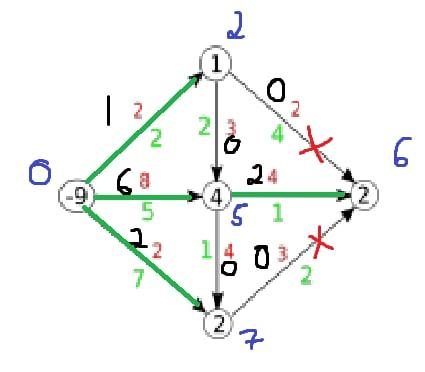
\includegraphics[width=.9\linewidth]{11.jpg}
\end{center}

\newpage
Iremos aumentar o valor da aresta BC, pois seguir o caminho AB-BC nos dá um custo menor do que seguir o caminho AC. Para isso iremos diminuir o valor da aresta AC e aumentar o valor da aresta AB. O Valor de t será 1, pois seremos restringidos pelo máximo da aresta AB:
\begin{center}
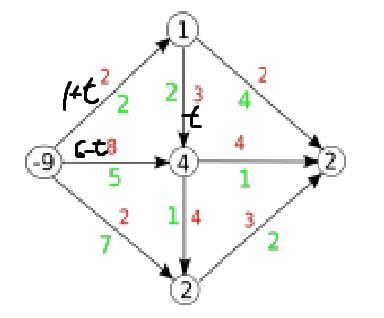
\includegraphics[width=.9\linewidth]{12.jpg}
\end{center}

\newpage
Temos agora o seguinte estado:
\begin{center}
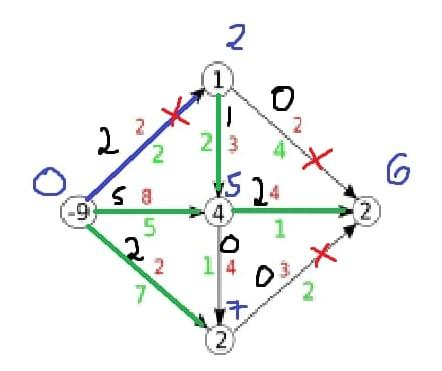
\includegraphics[width=.9\linewidth]{13.jpg}
\end{center}

\newpage
Agora iremos aumentar o valor da aresta CD, pois esse caminho tem custo menor do seguir o caminho AD. Para isso iremos aumentar junto o valor da aresta AC e diminuir o valor de AD. O valor de t é 2 pois seremos restringidos pelo mínimo (0) da aresta AD:
\begin{center}
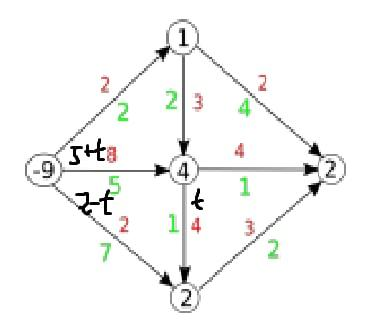
\includegraphics[width=.9\linewidth]{14.jpg}
\end{center}

\newpage
Temos agora o seguinte estado. Podemos perceber que temos 4 arestas fora da base. AB não pode ser alterada, pois ela é o único jeito de chegar em B e também faz parte do caminho mais eficiente para chegar em C, como vimos no primeiro passo do algoritmo. A aresta BE não vale a pena ser alterada, pois o Y de E é 6 e esse caminho também tem custo 6, logo não vale a pena mudar. A aresta AD não vale a pena ser alterada, pois o Y de D é 6 e o valor da aresta é 7. A aresta DE não vale apena ser alterada, pois ela nos dá um caminho que chega em E com custo 8 e o Y de E é 6. Logo, temos a solução ótima.
\begin{center}
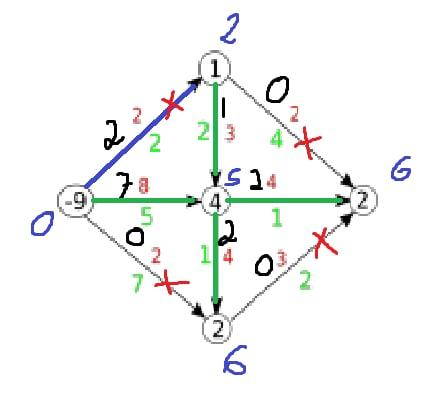
\includegraphics[width=.9\linewidth]{15.jpg}
\end{center}

Essa é, então, a solução ótima.

\newpage
\section{Questão 2}
\label{sec:org9589e0c}
Começamos com o seguinte estado:
\begin{center}
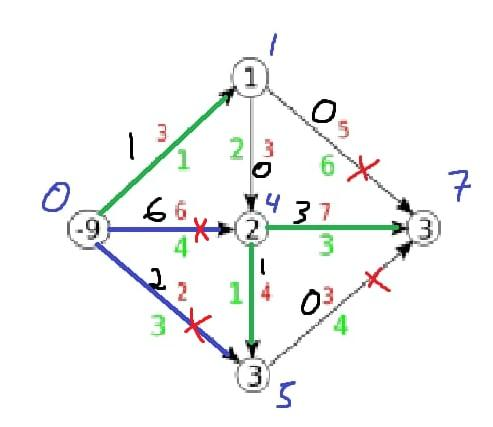
\includegraphics[width=.9\linewidth]{21.jpg}
\end{center}

\newpage
Iremos aumentar o valor do aresta BC, pois esse caminho chega em C com custo menor que AC. Para isso iremos aumentar AB e diminuir AC junto. O valor de t será 2, pois seremos restringidos pelo máximo da aresta AB:
\begin{center}
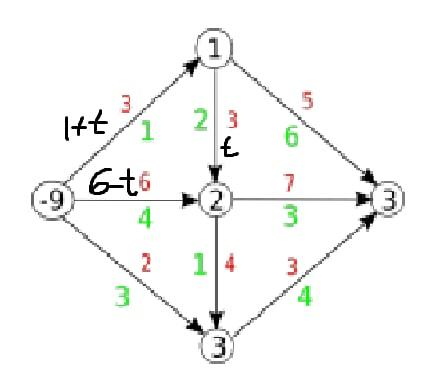
\includegraphics[width=.9\linewidth]{22.jpg}
\end{center}

\newpage
Agora, temos 4 arestas fora da base. Não vale a pena alterar AB como já foi visto no primeiro passo que fiz. Não vale a pena alterar o valor de BE, pois essa aresta nos dá um caminho de custo 7 para E, e o Y de E já é 7. Não vale a pena alterar o valor de AD pois essa aresta chega em D com custo 3 e o Y de D é 5, ou seja, vale a pena usarmos o máximo possível a aresta AD. Não vale a pena alterar o valor de DE, pois DE chega em E com custo 9 e o Y de E é 7. Logo, temos a solução ótima.
\begin{center}
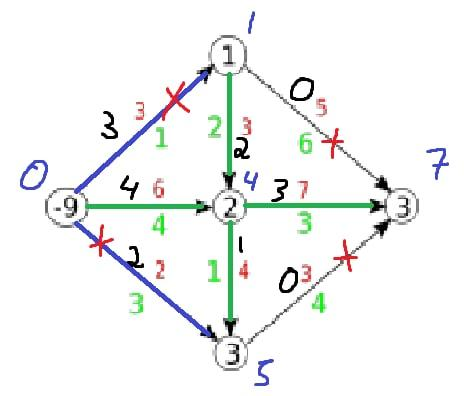
\includegraphics[width=.9\linewidth]{23.jpg}
\end{center}

\newpage
\section{Questão 3}
\label{sec:org8f214be}
Começamos com o seguinte estado:
\begin{center}
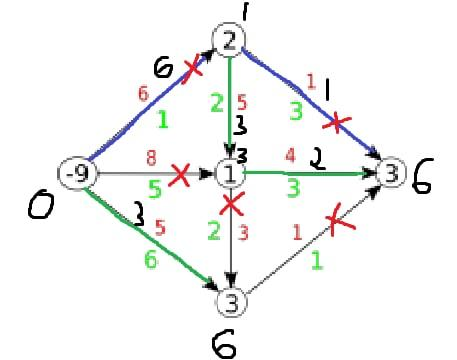
\includegraphics[width=.9\linewidth]{31.jpg}
\end{center}

Temos 5 arestas fora da base. Não vale a pena alterar AB, pois ela faz parte do caminho mais eficiente para chegar em C, em E e em B. Não vale a pena alterar BE pois é a aresta que chega de maneira mais eficiente em E, com total 4. Não devemos alterar AC pois ela chega em C com custo 5 e o Y de C é 3. Não devemos alterar CD, pois ela nos dá um caminho para chegar em C com custo 7, cujo y é 6. Por fim, não devemos alterar DE, pois ela nos faria chegar em E com custo 7 e o Y de E é 6. Logo, temos a solução ótima.
\end{document}